% <- percent signs are used to comment
\documentclass[12pt]{article}

%%%%%% PACKAGES - this part loads additional material for LaTeX %%%%%%%%%
% Nearly anything you want can be done in LaTeX if you load the right package 
% (search ctan.org or google it if you are looking for something).  We will load
% here a few that we need for this document or that we expect you to need later.

% The next 3 lines are needed to fix shortcomings of TeX that only make sense given its 40-year history ...
% Simple keep and ignore.
\usepackage[utf8]{inputenc}
\usepackage[T1]{fontenc}
\usepackage{lmodern}
\usepackage{amsmath}
\usepackage{changepage}
\usepackage{lipsum}

% Custom margins (and paper sizes etc.) because LaTeX else wastes much space
\usepackage[margin=1in]{geometry}

% The following packages are created by the American Mathematical Society (AMS)
% and provide lots of tools for special fonts, symbols, theorems, and proof
\usepackage{amsmath,amsfonts,amssymb,amsthm}
% mathtools contains many detail improvements over ams and core tex
\usepackage{mathtools}

% graphicx is required for images
\usepackage{graphicx}

% enumitem used for customizing enumerations
\usepackage[shortlabels]{enumitem}

% tikz is the package used for drawing, in particular for drawing trees. You may also find simplified packages like tikz-qtree and forest useful
\usepackage{tikz}

% hyperref allows links, urls, and many other PDF tricks.  We load it here
%          in such a way that the PDF file has info about it
\usepackage[%
	pdftitle={CS240 Assignment 0},%
	hidelinks,%
]{hyperref}


%%%%%% COMMANDS - here you can define your own LaTeX-commands %%%%%%%%%

%%%%%% End of Preamble %%%%%%%%%%%%%

\begin{document}

\begin{center}
{\Large\textbf{CS240, Spring 2022}}\\
\vspace{2mm}
{\Large\textbf{Assignment 3: Question 5}}\\
\vspace{3mm}
\end{center}
\begin{adjustwidth}{0em}{0pt}
\textbf{Q5b)} 
\begin{figure}[tbhp]
	\begin{center}
		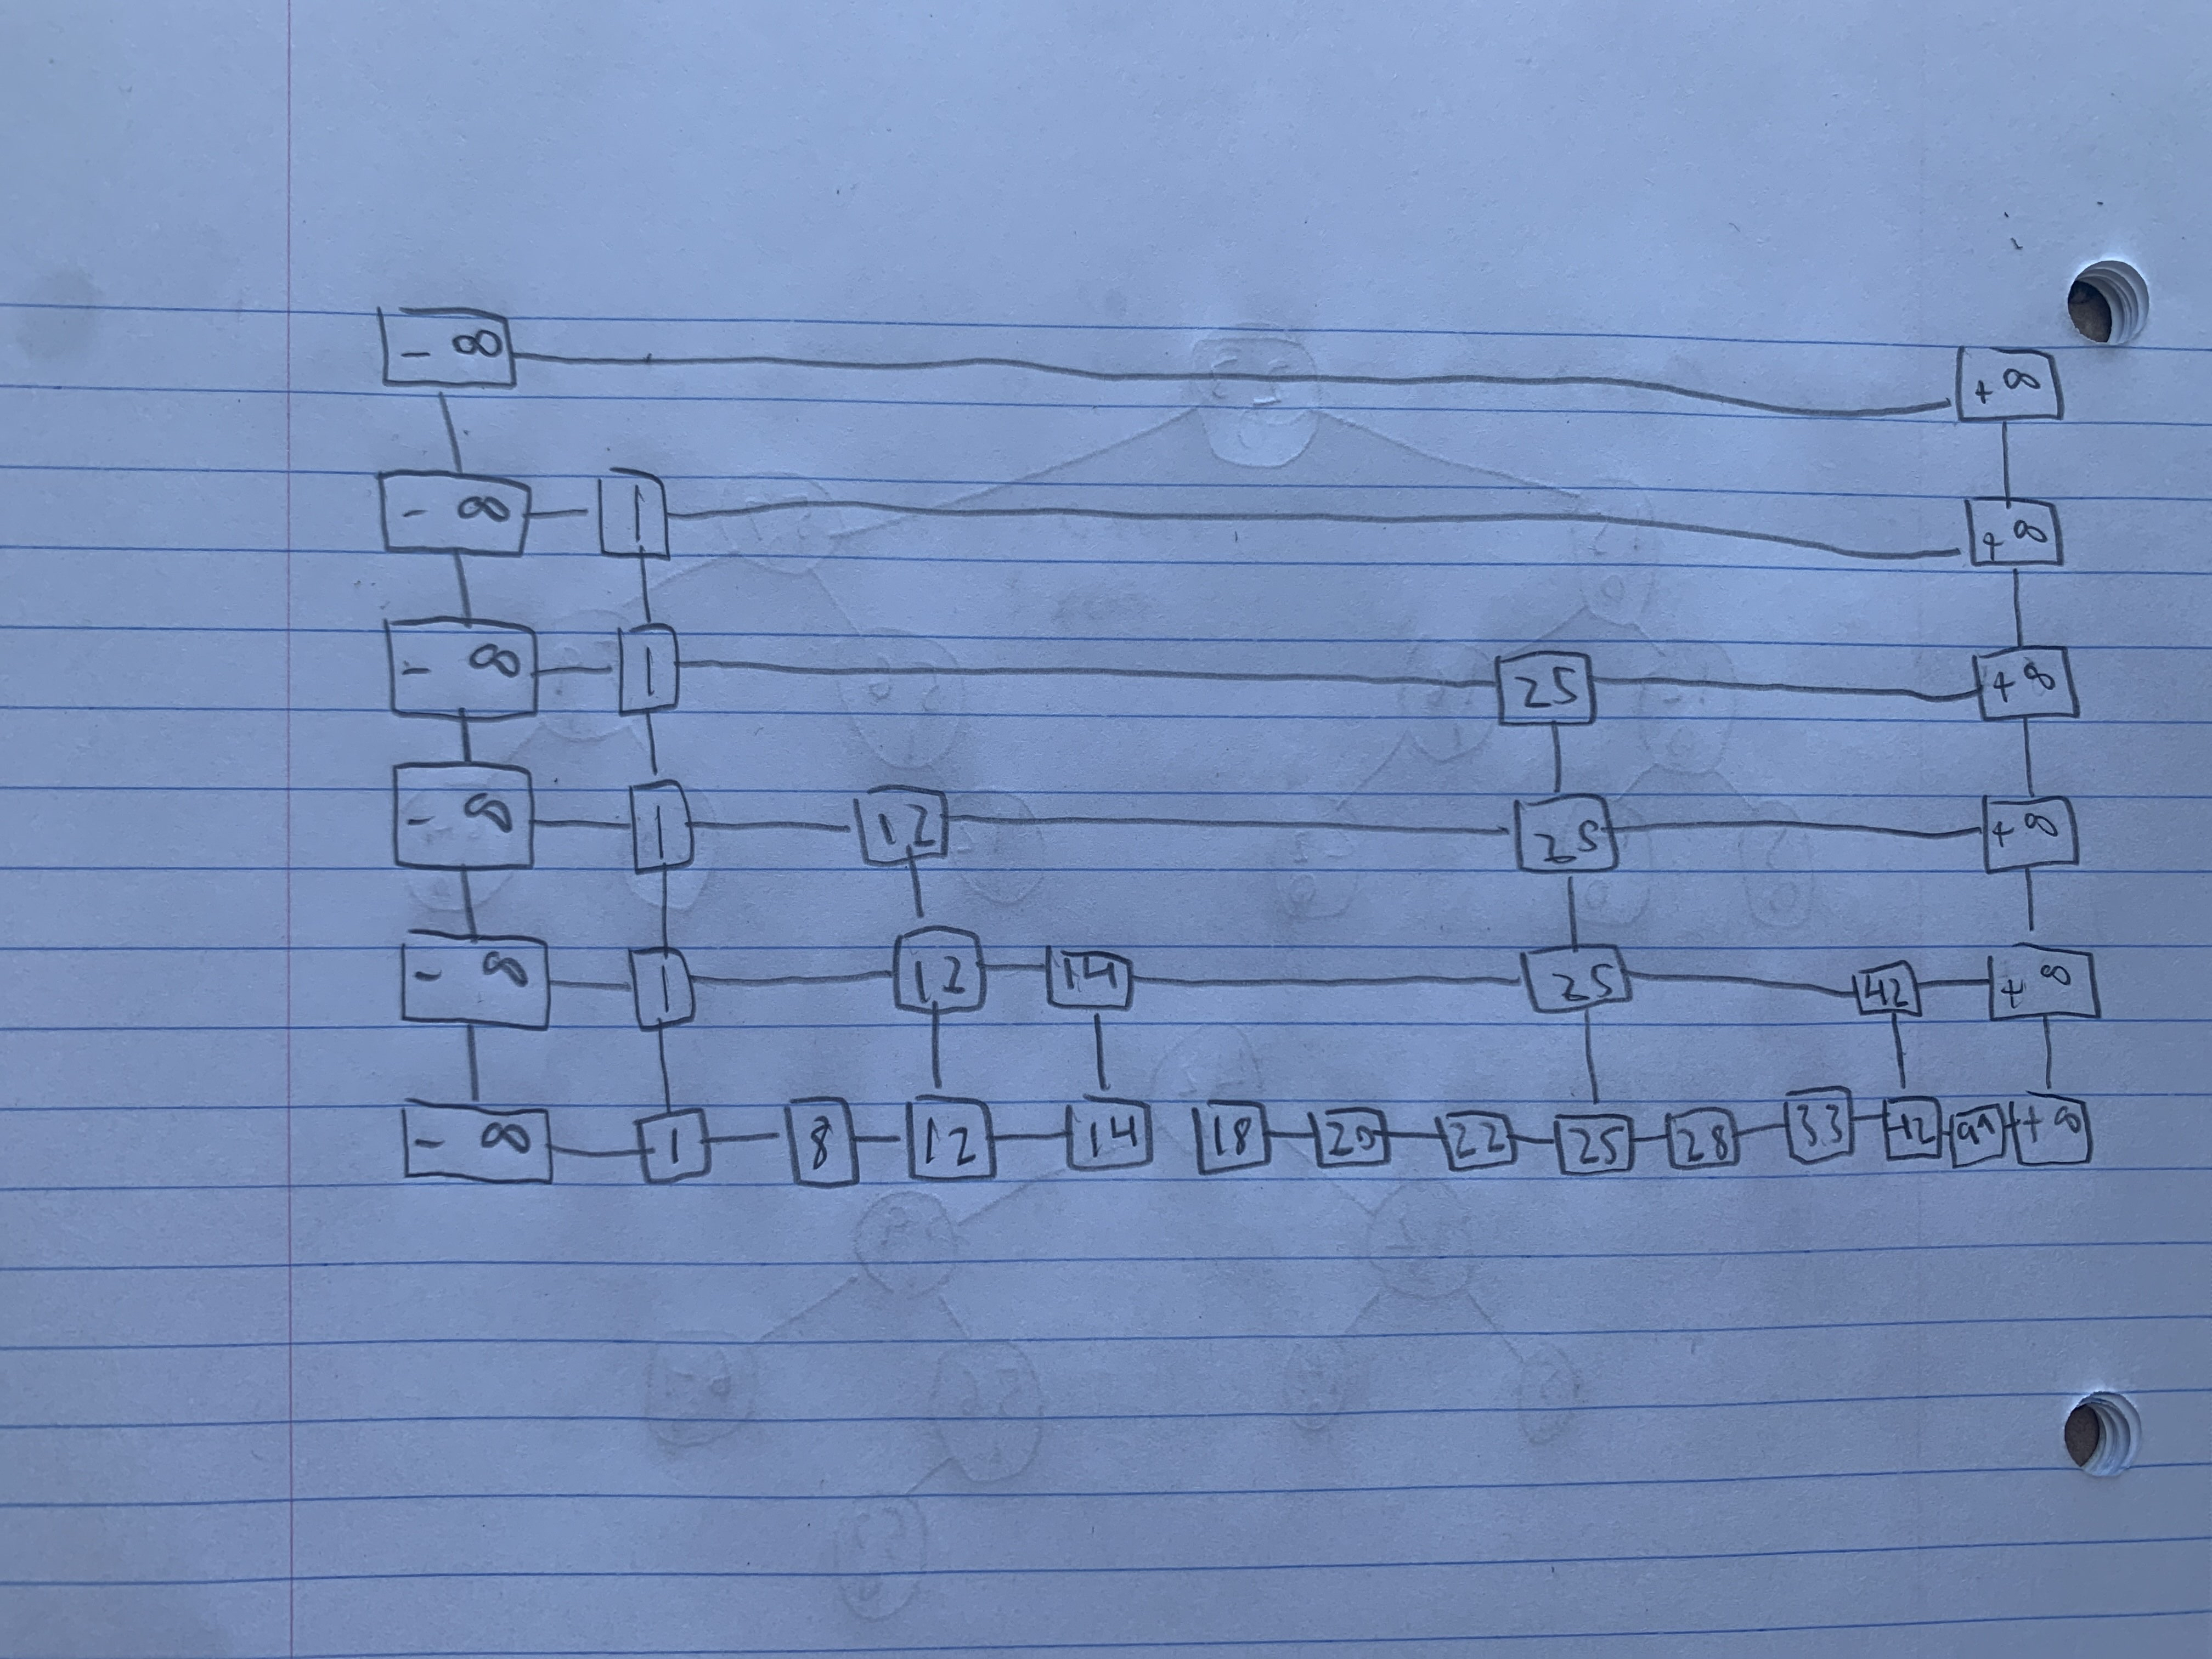
\includegraphics[width=0.8\textwidth, angle=0]{1.jpg}
	\end{center}
\end{figure}

\begin{center}
\begin{tabular}{| c || c c c c c c|} 
 \hline
 Key & 28 & 42 & 8 & 1 & 22 & 99  \\
 \hline
 Comparisons & 8 & 9 & 7 & 7 & 11 & 9  \\ 
 \hline
\end{tabular}
\end{center}
\textbf{Q5c)} We are told from the lectures that the height of the tower is given by the number of coin flips until you get a tails. In other words
\[ \text{height of tower = } \text{number of heads before a tails} \] 
We can reorganize this to get:
\[ \text{probability tower of height i = } \text{probability of i heads} \] 
We are told in the question that $p$ represents the probability of adding a new layer to the tower, in other words this means $p$ = probability of rolling heads. Since the probability of each coin flip is independent we get:
\[ \text{probability tower of height i = } p^i \] 
\end{adjustwidth} 
\newpage
\begin{adjustwidth}{0em}{0pt}
\textbf{Q5d)}
For each element in the skip list, the expected number of nodes is given by:
\[ = i*p^i \]
Since there are n elements in the skip list we know our space complexity will be proportional to: 
\[ = n*i*p^i \]
From e) we are given that the max height of the the list is log(n), therefore  if we know that $i$ can be the values from [0, ..., log(n)]. Thus our expected space complexity is given by:
\[ = \frac{1}{\log(n)}\sum^{\log(n)}_{i=0}n*i*p^i \]
\[ = \frac{n}{\log(n)}\sum^{\log(n)}_{i=0}i*p^i \]
Note that since $p$ is always less then 1, it follows that $i*p^i <= \frac{i}{log(n)}$, thus it follows that:
\[ \leq \frac{n}{\log(n)}\sum^{\log(n)}_{i=0}\frac{i}{log(n)} \]
\[ = \frac{n}{\log(n)}\frac{log(n)*(log(n)-1)}{2\log(n)} \]
Simplifying we get:
\[ \frac{n}{2} - \frac{n}{2\log{n}} \in O(n) \]
which proves out space complexity will be linear. \\ \\ 
\textbf{Q5e)}
For each element in the skip list, the number of elements with a height of $i$ or greater is given by:
\[ E(height) = n*p^i \]
We will create an indicator variable such that:
\[
 I(i) = \begin{array}{lr}
        0, & \text{if no elements have height i } 0\leq n\leq 1\\
        1, & \text{if some elements have height i } 0\leq n\leq 1
        \end{array}
\]
It thus follows that the height can be solved by finding:
\[ = 1 + \sum^{\infty}_{i=1} I(i) \]
Since n is a power of $\frac{1}{p}$ we can split this summation into 2 parts:
\[ = 1 + \sum^{log_{\frac{1}{p}}(n)}_{i=1} I(i) + \sum^{\infty}_{i= \log_{\frac{1}{p}}^n} I(i) \]
Using the equation for probability of a height we had at the top, our equation thus becomes:
\[ = 1 + \sum^{log_{\frac{1}{p}}(n)}_{i=1} 1 + \sum^{\infty}_{i= \log_{\frac{1}{p}}^n} n*p^i \]
Which then becomes:
\[ = 1 + log_{\frac{1}{p}}(n) + p*\sum^{\infty}_{i= \log_{\frac{1}{p}}^n} p^i \]
We can update the bounds to get:
\[ \text{height} <= 1 + log_{\frac{1}{p}}(n) + p*\sum^{\infty}_{i=0} p^i \]
By the taylor series we know that our infinite summation is equivalent to $\frac{1}{1-p}$ so w get:
\[ \text{height} <= 1 + log_{\frac{1}{p}}(n) + p*\frac{1}{1-p} \]
\[ \text{height} <= log_{\frac{1}{p}}(n) + \frac{1-p}{1-p} + p*\frac{1}{1-p} \]
\[ \text{height} <= log_{\frac{1}{p}}(n) + \frac{1}{1-p} \]
Which is as required.
\end{adjustwidth} 




\end{document}